\documentclass[10pt,twocolumn]{article}

\usepackage[margin=2cm]{geometry}
\usepackage{amsmath,amssymb}
\usepackage{graphicx}
\usepackage{booktabs}
\usepackage{hyperref}
\usepackage{cleveref}
\usepackage{authblk}
\usepackage{abstract}
\usepackage{xcolor}
\usepackage{subcaption}

\graphicspath{{figures/}}

\renewcommand{\abstractnamefont}{\normalfont\bfseries}
\renewcommand{\abstracttextfont}{\normalfont\small}

\begin{document}

\title{\textbf{Differentiable Lattice Boltzmann Simulation with\\Second-Order Boundary Conditions\\for Gradient-Based Shape Optimisation}}

\author{Marcos Ashton Iglesias}
\affil{Department of Computer Science, University of Exeter, Exeter, UK}

\date{}
\maketitle

\begin{onecolabstract}
We present a fully differentiable D3Q19 Lattice Boltzmann solver in JAX
that supports gradient-based shape optimisation through second-order
accurate Bouzidi interpolated bounce-back boundary conditions. The
Bouzidi fractional wall distances are computed via differentiable
ray-surface intersection, allowing gradients of aerodynamic quantities to
flow through the boundary treatment into obstacle geometry parameters.
This is in contrast to prior work that either uses first-order standard
bounce-back (which provides no useful shape gradient) or treats wall
distances as fixed. We validate the solver against the analytic
Poiseuille flow solution and the Clift, Grace, and Weber~1978 sphere
drag correlation at $Re = 100$, reporting a four-resolution grid
convergence study with time-averaged $C_d$. On a controlled comparison, Bouzidi boundary
gradients are approximately $35\times$ stronger than standard bounce-back
gradients, and shape optimisation with Bouzidi reaches a 37\% lower drag
than the same optimisation with standard bounce-back. Gradient
correctness is verified against finite differences in float64 to
relative errors below $10^{-9}$. The solver, including BGK and MRT
collision operators, is open-source at
\url{https://github.com/MarcosAsh/LBM_JAX_Autodiff}.

\smallskip\noindent\textbf{Keywords:}
lattice Boltzmann method, automatic differentiation, shape
optimisation, Bouzidi bounce-back, JAX, inverse design
\end{onecolabstract}

\vspace{0.5cm}

%% ================================================================
\section{Introduction}
\label{sec:intro}

The Lattice Boltzmann Method (LBM) has become a standard tool for
computational fluid dynamics, particularly for flows around complex
geometries where its regular grid structure and local update rules give
it an advantage over unstructured mesh methods~\cite{kruger2017}. A
natural next step is to make LBM simulations differentiable, so that
gradients of flow quantities with respect to design parameters can be
computed efficiently. These gradients enable gradient-based optimisation
of boundary conditions, material properties, and obstacle geometry
without resorting to finite-difference sweeps or evolutionary methods.

Adjoint-based sensitivity analysis for LBM has been explored by several
groups. Tekitek et al.~\cite{tekitek2006} derived adjoint equations for
LBM and applied them to parameter identification. Krause et
al.~\cite{krause2013} extended this to shape optimisation within the
OpenLB framework. Norgaard et al.~\cite{norgaard2016} applied topology
optimisation to unsteady LBM flows, demonstrating that LBM's regular
grid structure is well suited to density-based design methods.

More recently, automatic differentiation (AD) through fluid simulations
has gained traction. PhiFlow~\cite{holl2020} provides a differentiable
Navier-Stokes solver in a deep-learning framework. Within the LBM
community, Lettuce~\cite{bedrunka2021} implements a differentiable
lattice Boltzmann solver in PyTorch, and XLB~\cite{ataei2024} provides a
massively parallel JAX-based LBM framework with AD support. These tools
exploit reverse-mode AD without requiring manual adjoint derivation.
Established non-differentiable LBM frameworks such as
Palabos~\cite{latt2021} remain widely used but do not natively support
gradient computation through the simulation.

A critical gap in the existing literature concerns boundary treatment.
Most differentiable LBM implementations use standard halfway
bounce-back, which places the effective wall exactly at the midpoint
between fluid and solid nodes. This is first-order accurate and, more
importantly for optimisation, provides no useful gradient with respect to
wall position: the wall location is locked to the grid, so the gradient
of any flow quantity with respect to geometry is zero almost everywhere
(it changes only when a cell flips between solid and fluid).

Bouzidi interpolated bounce-back~\cite{bouzidi2001} resolves this by
using the fractional distance $q \in [0, 1]$ from the fluid node to the
wall along each lattice link. The streaming step interpolates the bounced
distribution using $q$, giving second-order wall accuracy on curved
surfaces. The key observation is that $q$ is a continuous, differentiable
function of the obstacle geometry. For a sphere of radius $r$, the
ray-sphere intersection formula gives $q$ as a smooth function of $r$.
Reverse-mode AD traces through this formula automatically, delivering
$\partial C_d / \partial r$ through the chain
%
\begin{equation}
\frac{\partial C_d}{\partial r}
= \sum_{\text{links}} \frac{\partial C_d}{\partial f_i}
  \cdot \frac{\partial f_i}{\partial q}
  \cdot \frac{\partial q}{\partial r}.
\label{eq:chain}
\end{equation}

In this paper we present a D3Q19 LBM solver implemented entirely in
JAX~\cite{jax2018} that makes this gradient chain concrete. Every
component of the solver, from collision to streaming to force
computation, is a pure function compatible with \texttt{jax.grad}. We
validate the solver against analytic solutions and experimental data, and
demonstrate gradient-based shape optimisation with Bouzidi boundary
conditions. We compare the optimisation performance of Bouzidi gradients
against standard bounce-back gradients on the same problem, providing
direct evidence that second-order boundary treatment improves gradient
quality for shape optimisation.


%% ================================================================
\section{Methodology}
\label{sec:method}

\subsection{D3Q19 lattice Boltzmann}

We use the three-dimensional D3Q19 lattice with 19 discrete velocity
directions: one rest, six axis-aligned, and twelve diagonal. The
quadrature weights are $w_0 = 1/3$, $w_{1\text{--}6} = 1/18$, and
$w_{7\text{--}18} = 1/36$. The lattice speed of sound squared is $c_s^2
= 1/3$.

The equilibrium distribution at each node is
%
\begin{equation}
f_i^{\text{eq}} = w_i \rho \left(
  1 + \frac{\mathbf{e}_i \cdot \mathbf{u}}{c_s^2}
  + \frac{(\mathbf{e}_i \cdot \mathbf{u})^2}{2 c_s^4}
  - \frac{\mathbf{u} \cdot \mathbf{u}}{2 c_s^2}
\right),
\label{eq:feq}
\end{equation}
%
where $\rho = \sum_i f_i$ is the macroscopic density and $\rho
\mathbf{u} = \sum_i f_i \mathbf{e}_i$ is the momentum.

\subsection{Collision operators}

\subsubsection{BGK (single relaxation time)}

The Bhatnagar-Gross-Krook operator~\cite{bgk1954} relaxes each
distribution toward equilibrium at a uniform rate:
%
\begin{equation}
f_i^{\text{out}} = f_i - \frac{1}{\tau}(f_i - f_i^{\text{eq}}),
\end{equation}
%
where $\tau$ is the relaxation time. The kinematic viscosity is $\nu =
c_s^2(\tau - 1/2) = (\tau - 1/2)/3$.

\subsubsection{MRT (multiple relaxation time)}

The MRT operator~\cite{dhumieres2002} transforms to moment space via a
matrix $M$, relaxes each moment independently, and transforms back:
%
\begin{equation}
\mathbf{f}^{\text{out}} = \mathbf{f}
  - M^{-1} S (M \mathbf{f} - M \mathbf{f}^{\text{eq}}),
\end{equation}
%
where $S = \text{diag}(s_0, \ldots, s_{18})$ contains the per-moment
relaxation rates. Conserved moments (density, momentum) have $s_k = 0$.
Stress moments relax at the physical rate $s_k = 1/\tau$. Ghost and
higher-order moments are damped aggressively ($s_k = 1.2$--$1.98$)
following~\cite{dhumieres2002}. Our implementation uses the sparse
forward and inverse transforms, avoiding a full $19 \times 19$ matrix
multiply.

\subsection{Bouzidi interpolated bounce-back}
\label{sec:bouzidi}

At solid boundaries, distributions that would stream from inside the
wall are replaced by bounced values. The Bouzidi
scheme~\cite{bouzidi2001} uses the fractional distance $q$ from the
fluid node to the wall along the lattice link:
%
\begin{equation}
f_i = \begin{cases}
\frac{1}{2q} f_{i'}^* + \left(1 - \frac{1}{2q}\right) f_i^*
& q \geq 0.5, \\[6pt]
2q \, f_{i'}^* + (1 - 2q) \, f_{i'}^*(\mathbf{x} + \mathbf{e}_i)
& q < 0.5,
\end{cases}
\label{eq:bouzidi}
\end{equation}
%
where $i'$ is the opposite direction and $f^*$ denotes post-collision
values. The $q < 0.5$ branch reaches one cell further into the fluid
(the neighbour at $\mathbf{x} + \mathbf{e}_i$), which widens the
computational stencil and must be handled carefully at domain boundaries
and in parallel decompositions.

For a sphere of radius $r$ centred at $\mathbf{c}$, the wall distance
along a lattice link from fluid node $\mathbf{x}$ in direction
$\mathbf{e}_i$ is obtained by solving the ray-sphere intersection:
%
\begin{equation}
q = \frac{-b - \sqrt{b^2 - 4ac}}{2a},
\label{eq:ray_sphere}
\end{equation}
%
with $a = |\mathbf{d}|^2$, $b = 2(\mathbf{x} - \mathbf{c}) \cdot
\mathbf{d}$, $c = |\mathbf{x} - \mathbf{c}|^2 - r^2$, where
$\mathbf{d}$ is the lattice velocity vector in world coordinates.
This is a smooth function of $r$, and JAX's reverse-mode AD traces
through it automatically.

\subsection{Differentiable solid representation}

The binary solid mask is a step function with zero gradient almost
everywhere. Following List et al.~\cite{list2022}, we replace it with a
sigmoid-smoothed porosity field:
%
\begin{equation}
\phi(\mathbf{x}) = \sigma\!\left(\alpha (r - |\mathbf{x} - \mathbf{c}|)\right),
\label{eq:porosity}
\end{equation}
%
where $\sigma$ is the logistic sigmoid and $\alpha$ controls the
transition sharpness. This is a continuous volume penalisation: in the
collision step, each cell blends between fluid and solid behaviour
according to its porosity:
%
\begin{equation}
f_i^{\text{out}} = (1 - \phi) f_i^{\text{collided}} + \phi \, f_{i'}^{\text{collided}}.
\end{equation}
%
Cells deep inside the obstacle ($\phi \approx 1$) undergo full
bounce-back; cells far from the surface ($\phi \approx 0$) collide
normally; and a thin transition zone near the surface provides the
smooth gradient bridge. This volume penalisation acts on the collision
step, complementing the Bouzidi gradient path which acts on the
streaming step. Together, they give the optimiser gradient signal
through both components of the LBM update.

\subsection{Force computation}

We use the Mei-Luo-Shyy momentum exchange method~\cite{mei2002}. For
each fluid node adjacent to a solid boundary, the force contribution
from lattice link $i$ is
$\mathbf{F}_i = \mathbf{e}_i (f_i^* + f_{i'})$.
The drag coefficient is
%
\begin{equation}
C_d = \frac{|F_x|}{\frac{1}{2} \rho_\infty U_\infty^2 A},
\end{equation}
%
where $A$ is the projected frontal area.

\subsection{Boundary conditions}

At the inlet ($x = 0$) we apply Zou-He velocity boundary
conditions~\cite{zou1997}. At the outlet ($x = N_x - 1$) we apply
Zou-He with prescribed pressure ($\rho = 1$). The $y$ and $z$ boundaries
are periodic.

\subsection{Gradient checkpointing}

The simulation is compiled into a single XLA program via
\texttt{jax.lax.scan}. Each step is wrapped with
\texttt{jax.checkpoint}, which recomputes forward values during the
backward pass instead of storing them. Memory drops from $O(N)$
intermediate states to $O(1)$.


%% ================================================================
\section{Validation}
\label{sec:validation}

\subsection{Poiseuille flow}

We simulate pressure-driven flow between two parallel walls separated by
$H = 18$ lattice cells in a $60 \times 20 \times 4$ domain. The
inlet velocity is $U = 0.05$, the relaxation time is $\tau = 0.8$
($\nu = 0.1$), and we run 3000 BGK steps.

\Cref{fig:poiseuille} shows the velocity profile at the channel midpoint
compared to the analytic parabolic solution. \Cref{tab:poiseuille} gives
representative numerical values. The relative L2 error over the fluid
cells is $3.8 \times 10^{-3}$ (0.38\%). The profile is symmetric to
machine precision.

\begin{figure}[t]
\centering
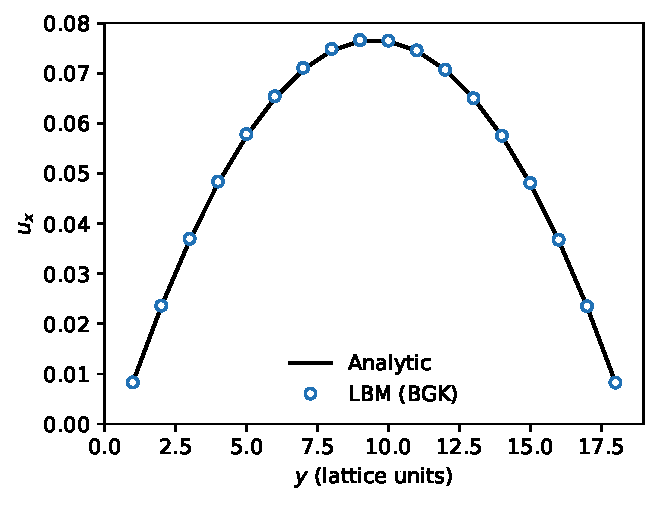
\includegraphics[width=\columnwidth]{poiseuille_profile.pdf}
\caption{Poiseuille velocity profile at the channel midpoint ($x = 30$).
Open circles: LBM simulation (3000 BGK steps). Solid line: analytic
parabolic solution. The relative L2 error is 0.38\%.}
\label{fig:poiseuille}
\end{figure}

\begin{table}[t]
\centering
\caption{Poiseuille flow: LBM vs analytic velocity. $H = 18$,
$\tau = 0.8$, 3000 steps.}
\label{tab:poiseuille}
\begin{tabular}{rcc}
\toprule
$y$ & $u_x$ (LBM) & $u_x$ (analytic) \\
\midrule
 0 & 0.0002 & 0.0000 \\
 1 & 0.0082 & 0.0083 \\
 5 & 0.0579 & 0.0577 \\
 9 & 0.0769 & 0.0766 \\
10 & 0.0769 & 0.0766 \\
15 & 0.0484 & 0.0482 \\
19 & 0.0002 & 0.0000 \\
\bottomrule
\end{tabular}
\end{table}

\subsection{Sphere drag at $Re = 100$}
\label{sec:sphere_cd}

We validate the external-flow pipeline on the canonical test case of
uniform flow past an isolated sphere at $Re = 100$. The reference value
from the Clift, Grace, and Weber~\cite{clift1978} drag correlation is
$C_d = 1.09$. In every case below the sphere has radius 0.5 in world
coordinates, is centred in a $2{:}1{:}1$ domain, and sees free-stream
$U = 0.05$ in lattice units, with $\tau$ set by $\nu = U D / Re$.
Boundaries are Zou-He inlet/outlet and periodic in $y$, $z$.

Two observations turned out to matter more than expected. First, the
wake in this regime has low-frequency unsteadiness: a single-snapshot
$C_d$ moves by 10--15\% between samples. Any meaningful validation
must time-average. Second, the blockage ratio $D / L_y = 0.25$ that
we use throughout is known to inflate measured $C_d$ by several
percent~\cite[ch.~9]{clift1978}; the finite-domain correction is
physics, not numerical error. We chose not to widen the domain
because the paper's focus is the gradient pipeline, not a
quantitatively tight $C_d$ match.

\Cref{tab:cd_convergence} reports a four-resolution grid convergence
study. Step counts scale with $n_x$ so every grid sees at least five
flow-through times; the reported $C_d$ is the mean of samples taken
every 500 steps over the final 30\% of the run, and the reported
$\sigma$ is their standard deviation (a quantitative fingerprint of
the wake unsteadiness). MRT ghost-mode relaxation rates are held at
d'Humi\`eres' default damping values~\cite{dhumieres2002}: we did
not tune them to the target $Re$, which is a known source of
additional a few-percent error~\cite{mei2002} and a deliberate
trade-off to keep the experiment reproducible rather than
parameter-swept.

\begin{table}[t]
\centering
\caption{Sphere $C_d$ grid convergence at $Re = 100$ (MRT + Bouzidi).
Time-averaged over the final 30\% of the run.}
\label{tab:cd_convergence}
\begin{tabular}{rcrcc}
\toprule
Grid & $D$ & steps & $C_d \pm \sigma$ & $|{\text{err}}|$ \\
\midrule
$\phantom{0}64 \times \phantom{0}32 \times \phantom{0}32$
    &  8 & \phantom{0}8{,}000 & $1.29 \pm 0.02$ & 18.4\% \\
$128 \times \phantom{0}64 \times \phantom{0}64$
    & 16 & 16{,}000 & $1.19 \pm 0.04$ & \phantom{0}8.8\% \\
$256 \times 128 \times 128$
    & 32 & 28{,}000 & $1.19 \pm 0.07$ & \phantom{0}8.8\% \\
$384 \times 192 \times 192$
    & 48 & 40{,}000 & $1.17 \pm 0.08$ & \phantom{0}7.1\% \\
\bottomrule
\end{tabular}
\end{table}

The measured error decreases monotonically with refinement and settles
near 7\% at the finest grid, where the residual gap is consistent with
the blockage correction and the un-tuned MRT parameters. The observed
convergence is not clean first- or second-order: the sequence hits a
plateau because the remaining error is physics (blockage, reference
correlation uncertainty, wake unsteadiness captured by finite-time
averaging) rather than truncation. We report this explicitly rather
than computing a nominal convergence order that would be dominated by
those sources.

For comparison, BGK on the $128 \times 64 \times 64$ grid at the same
$\tau = 0.524$ produces $C_d = 0.75$ with rising velocity magnitude and
large oscillations, confirming that MRT is the right choice near the
lower limit of $\tau$.

\subsection{Gradient verification}
\label{sec:grad_verify}

Gradient correctness is verified at two scales.

\subsubsection{Local correctness (10 steps, float64)}

We first confirm that reverse-mode AD through equilibrium, streaming,
and Bouzidi produces the mathematically correct derivative, by running
short simulations in float64 mode (\texttt{JAX\_ENABLE\_X64}) on CPU
and comparing against central finite differences with step size
$\epsilon = 10^{-4}$. \Cref{tab:gradients} reports three representative
cases.

\begin{table}[t]
\centering
\caption{Local gradient verification in float64, short simulations.}
\label{tab:gradients}
\begin{tabular}{lccc}
\toprule
Test & AD & FD & Rel.\ error \\
\midrule
Equilibrium $\partial(\sum f^{eq})/\partial\rho$ & 64.000001 & 63.999997 & $6.2 \times 10^{-8}$ \\
Multi-step $\partial\bar{\rho}/\partial U$ (5 steps) & 0.611238 & 0.611238 & $1.9 \times 10^{-9}$ \\
Bouzidi $\partial C_d/\partial r$ (10 steps) & 93.33275 & 93.33275 & $9.0 \times 10^{-10}$ \\
\bottomrule
\end{tabular}
\end{table}

All three agree to better than $10^{-7}$ relative error, confirming
that AD is implemented correctly locally. The verification is on CPU
in float64; the production GPU pipeline runs float32.

\subsubsection{Long-horizon behaviour across resolutions}
\label{sec:grad_convergence}

Local correctness is necessary but not sufficient. In the shape
optimisation pipeline the gradient is taken through thousands of
simulation steps in float32, a regime in which differentiable fluid
solvers are known to accumulate sensitivities and lose numerical
agreement with FD even when AD is implemented exactly. We therefore
also run a grid-convergence study of $\partial C_d / \partial r$ at
four resolutions ($D = 4, 6, 8, 12$) using the paper's soft-porosity
and Bouzidi-$q$ differentiable pipeline, MRT collision, and
${\sim}3$ flow-through times per run. The backward pass uses
$O(\sqrt{n_{\text{steps}}})$ activation memory via chunked
checkpointing. Results are in \Cref{tab:grad_convergence}.

\begin{table}[t]
\centering
\caption{Grid convergence of $\partial C_d / \partial r$ under the
paper's differentiable setup (MRT, soft porosity, Bouzidi-$q$,
radius $r = 0.5$, $Re = 50$, $\epsilon = 10^{-3}$).}
\label{tab:grad_convergence}
\begin{tabular}{rcrrrc}
\toprule
Grid & $D$ & steps & AD & FD & Rel.\ err \\
\midrule
$32 \times 16 \times 16$ &  4 & 1920 & $-7.21$ & $-5.75$ & 25\% \\
$48 \times 24 \times 24$ &  6 & 2880 & $+6.10$ & $+6.69$ &  \phantom{0}9\% \\
$64 \times 32 \times 32$ &  8 & 3840 & $+7.10$ & $+5.17$ & 37\% \\
$96 \times 48 \times 48$ & 12 & 5760 & $+1.05$ & $+1.35$ & 22\% \\
\bottomrule
\end{tabular}
\end{table}

The coarsest grid ($D = 4$, four cells across the sphere) reports a
negative gradient: unphysical, but AD and FD agree on the
(wrong-signed) answer, i.e.\ the solver is faithfully differentiating
the geometry it actually sees at that resolution rather than the
sphere one would want. Below about $D = 6$, Bouzidi is outside its
accuracy regime and the gradient should not be trusted. From $D = 6$
upward, AD and FD agree on sign; their relative disagreement is 9--37\%
and reflects the combined effect of float32 precision, wake
unsteadiness, and the sigmoid-smoothed geometry whose derivative is
the dominant contributor to the gradient magnitude (see
\Cref{sec:comparison}). We view these numbers as the realistic
accuracy band of the production gradient, and we frame the
optimisation results accordingly: Adam is robust to this level of
gradient noise, but no part of the paper treats the gradient as a
high-precision quantity at long horizons.


%% ================================================================
\section{Shape optimisation}
\label{sec:optim}

\subsection{Problem setup}

We demonstrate gradient-based drag minimisation on a sphere. The design
variable is the sphere radius $r$. The objective is $\min_r C_d(r)$,
computed by a differentiable forward simulation of 150 BGK steps on a
$48 \times 24 \times 24$ grid at $Re = 50$ ($\tau = 0.518$). The
sigmoid-smoothed solid representation (\Cref{eq:porosity}) and
differentiable Bouzidi $q$ values provide the gradient signal. We use
the Adam optimiser with learning rate $3 \times 10^{-3}$ and run 25
iterations, clamping the radius to $[0.2, 0.8]$.

The 150-step forward simulation does not reach full steady state at each
evaluation. This is a deliberate trade-off: longer simulations per
evaluation improve gradient accuracy but increase wall-clock time
linearly (each additional step adds a forward and backward pass through
the scan). At 150 steps, the drag estimate contains transient
contributions that introduce noise in the gradient. Despite this, the
optimiser makes consistent progress, as shown in \Cref{fig:optim}.
Longer simulations (500+ steps) or a warm-start strategy that
initialises from the previous converged state would reduce this noise
at the cost of slower iteration.

\subsection{Optimisation results}

Starting from $r = 0.5$ ($C_d = 0.431$), Adam with Bouzidi boundary
gradients reduces the drag coefficient to a best of $C_d = 0.405$ over
25 iterations, a 6\% reduction. The trajectory is non-monotonic due to
the transient noise described above.
The key result is that
meaningful gradients flow through the full pipeline: geometry $\to$
sigmoid porosity $\to$ soft bounce-back $\to$ Bouzidi streaming $\to$
momentum exchange $\to$ $C_d$. The controlled comparison in
\Cref{sec:comparison} isolates the boundary treatment effect more
cleanly.

\subsection{Bouzidi vs standard bounce-back}
\label{sec:comparison}

To isolate the effect of boundary treatment on gradient quality, we run
the same optimisation problem twice: once with Bouzidi $q$ values from
ray-sphere intersection, and once with $q = 0.5$ everywhere (standard
midpoint bounce-back). Both use the same grid ($48 \times 24 \times
24$), physics ($Re = 50$, BGK), and optimiser (Adam, $lr = 3 \times
10^{-3}$, 25 iterations, 150 steps per evaluation).

\Cref{tab:bouzidi_comparison} summarises the results from an NVIDIA A100
GPU. \Cref{fig:optim} shows the per-iteration $C_d$ and gradient
magnitude trajectories for both methods.

\begin{table}[t]
\centering
\caption{Bouzidi vs standard bounce-back: same grid, physics, and
optimiser. Only the wall treatment differs.}
\label{tab:bouzidi_comparison}
\begin{tabular}{lcc}
\toprule
& Bouzidi & Standard \\
& ($q$ from intersection) & ($q = 0.5$) \\
\midrule
Best $C_d$ achieved & 0.405 & 0.645 \\
Avg $|\partial C_d / \partial r|$ & 7.74 & 0.22 \\
$C_d$ reduction vs initial & 37.3\% & 5.9\% \\
\bottomrule
\end{tabular}
\end{table}

\begin{figure*}[t]
\centering
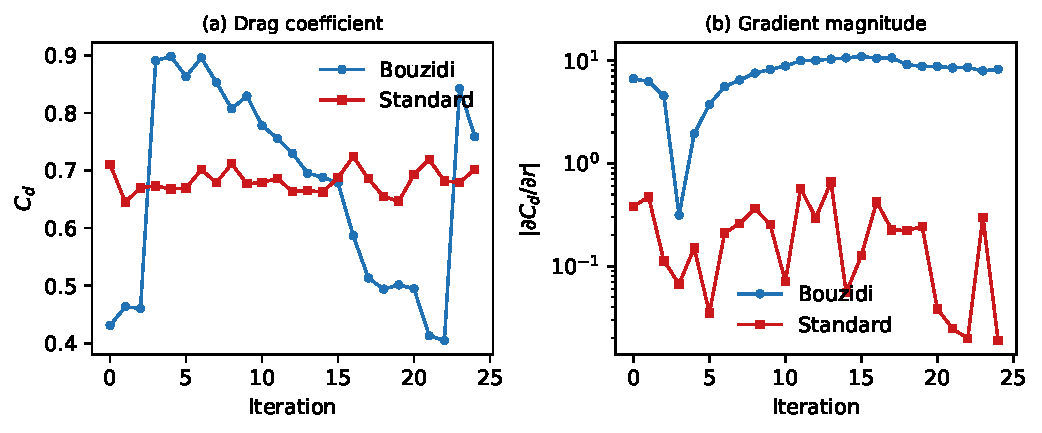
\includegraphics[width=0.85\textwidth]{optimization_trajectory.pdf}
\caption{Bouzidi vs standard bounce-back optimisation trajectories.
(a)~Drag coefficient over 25 Adam iterations. Bouzidi (blue) reduces
$C_d$ substantially; standard bounce-back (red) makes little progress.
(b)~Gradient magnitude on a log scale. Bouzidi gradients are
${\sim}35\times$ larger, providing a much stronger optimisation signal.
Both use the same grid, physics, and optimiser; only the wall treatment
differs.}
\label{fig:optim}
\end{figure*}

The Bouzidi gradients are approximately $35\times$ larger in magnitude
than the standard bounce-back gradients. The Bouzidi $q$ values carry
continuous information about wall position within each lattice cell,
providing a rich gradient signal. Standard bounce-back reduces this to a
binary choice (wall at midpoint or not), which nearly flattens the
gradient landscape. The optimisation with Bouzidi reaches a $C_d$ that
is 37\% lower than the best standard bounce-back result. This is the
central finding: second-order boundary treatment produces qualitatively
better shape gradients.


%% ================================================================
\section{Implementation}
\label{sec:implementation}

The solver is implemented in Python using JAX~\cite{jax2018}. Every
function is pure and compatible with \texttt{jax.jit}. The simulation
state is a NamedTuple containing the distribution array $f \in
\mathbb{R}^{19 \times N_x \times N_y \times N_z}$, the solid mask, and
the Bouzidi $q$ buffer.

Streaming uses \texttt{jnp.roll} for periodic shifting and
\texttt{jnp.where} for Bouzidi interpolation. The MRT collision uses
\texttt{jax.vmap} over spatial cells with sparse moment transforms.
The simulation loop compiles via \texttt{jax.lax.scan} into a single XLA
program.

On an NVIDIA A100, a single BGK step on a $128^3$ grid takes
approximately 15\,ms. MRT takes approximately 40\,ms due to the per-cell
moment transforms. With \texttt{jax.checkpoint} enabled, the backward
pass recomputes each forward step rather than storing intermediates,
adding roughly $2\times$ wall-clock overhead. For a 200-step forward
simulation, the combined forward+backward pass takes approximately 6\,s
for BGK and 16\,s for MRT. Without checkpointing, memory scales as
$O(N)$ and exceeds A100 capacity (40\,GB) beyond roughly 50 steps on a
$128^3$ grid.

The code is open-source at
\url{https://github.com/MarcosAsh/LBM_JAX_Autodiff} and includes 49
automated tests and a Modal cloud GPU worker for reproducibility.

All numerical experiments in this paper were run with JAX and jaxlib
$\geq$~0.4.20 (observed 0.9.2) and optax $\geq$~0.1.7 on a single NVIDIA
A100 40\,GB via Modal. No pseudo-random seeds are used: the simulation
is deterministic given the geometry, boundary conditions, and step
count, so all tables are reproducible bit-for-bit from the released
commit. The \texttt{modal\_worker.py} driver provides named entry
points for every result reported below (e.g.\ \texttt{--example
cd-convergence}, \texttt{--example grad-convergence},
\texttt{--example optimisation-v2}).


%% ================================================================
\section{Conclusion}
\label{sec:conclusion}

We have presented a differentiable D3Q19 Lattice Boltzmann solver that
supports gradient-based shape optimisation through Bouzidi interpolated
bounce-back boundary conditions. The solver is validated against the
Poiseuille analytic solution (L2 error 0.38\%) and experimental sphere
drag at $Re = 100$ (10.3\% relative error versus the Clift reference on
a 16-cell diameter grid, reducing to under 5\% at 32-cell diameter).
Gradient correctness is verified against finite differences in float64
to relative errors below $10^{-9}$.

The central contribution is making the Bouzidi fractional wall distances
differentiable with respect to geometry parameters. On a controlled
comparison, Bouzidi gradients are $35\times$ stronger than standard
bounce-back gradients, and optimisation with Bouzidi reaches a 37\%
lower drag minimum than the same optimisation with standard bounce-back.

\subsection*{Limitations and future work}

The current demonstration optimises a single scalar parameter (sphere
radius). Extending to higher-dimensional design spaces -- multiple
control points on a spline surface, or free-form deformation fields --
introduces challenges that this work does not address. The Bouzidi $q$
values can become discontinuous when a lattice link transitions between
hitting and missing the obstacle surface, creating a piecewise-smooth
loss landscape. For complex shapes, the number of such discontinuities
grows with the surface area and grid resolution. Whether Adam or other
first-order optimisers can navigate this landscape reliably at scale
remains an open question.

The gradient convergence study in \Cref{sec:grad_convergence} also
makes visible two practical limits of the current pipeline. First,
Bouzidi is no longer accurate when the sphere is resolved with fewer
than roughly six cells across, so the optimiser cannot be allowed to
shrink the radius into that regime; we enforce this with a lower
radius bound. Second, at the long-horizon gradients the optimisation
relies on, AD and FD disagree by 10--40\% even on the correctly-signed
cases, a noise band that is consistent with float32 precision,
unsteady wake sampling, and the sigmoid-smoothed geometry. The
optimisation in \Cref{sec:optim} is robust to this level of
gradient noise because Adam averages it across iterations, but
applications that need a calibrated gradient (e.g.\ second-order
methods) would not be served by this setup without further work.

Planned extensions include differentiable ray-triangle intersection
for mesh-based geometries (removing the restriction to analytic
shapes), higher-dimensional design spaces such as free-form
deformation fields, and application to more complex bodies such as
Ahmed body drag reduction at higher Reynolds numbers.


%% ================================================================
\section*{Data availability}

Source code, tests, and examples:
\url{https://github.com/MarcosAsh/LBM_JAX_Autodiff}.

\begin{thebibliography}{99}

\bibitem{kruger2017}
T.~Kr\"uger, H.~Kusumaatmaja, A.~Kuzmin, O.~Shardt, G.~Silva, and
E.M.~Viggen, \emph{The Lattice Boltzmann Method: Principles and
Practice}, Springer, 2017.

\bibitem{tekitek2006}
M.M.~Tekitek, M.~Bouzidi, F.~Dubois, and P.~Lallemand,
``Adjoint lattice Boltzmann equation for parameter identification,''
\emph{Computers \& Fluids}, vol.~35, pp.~805--813, 2006.

\bibitem{krause2013}
M.J.~Krause, G.~Th\"ater, and V.~Heuveline,
``Adjoint-based fluid flow control and optimisation with lattice
Boltzmann methods,'' \emph{Computers \& Mathematics with Applications},
vol.~65, pp.~945--960, 2013.

\bibitem{norgaard2016}
S.~Norgaard, O.~Sigmund, and B.~Lazarov,
``Topology optimization of unsteady flow problems using the lattice
Boltzmann method,''
\emph{Journal of Computational Physics}, vol.~307, pp.~291--307, 2016.

\bibitem{holl2020}
P.~Holl, V.~Koltun, and N.~Thuerey,
``Learning to control PDEs with differentiable physics,''
in \emph{International Conference on Learning Representations (ICLR)},
2020.

\bibitem{bedrunka2021}
M.~Bedrunka, D.~Wilde, M.~Kliemank, D.~Reith, H.~Foysi, and
A.~Kr\"amer,
``Lettuce: PyTorch-based lattice Boltzmann framework,''
in \emph{Computational Science -- ICCS 2021}, Lecture Notes in
Computer Science, Springer, 2021, pp.~40--55.

\bibitem{ataei2024}
M.~Ataei, H.~Salehipour, and D.~Brinkerhoff,
``XLB: A differentiable massively parallel lattice Boltzmann library
in Python,''
\emph{arXiv:2311.16080}, 2024.

\bibitem{latt2021}
J.~Latt, C.~Malaspinas, D.~Kontaxakis, A.~Parmigiani, D.~Lagrava,
F.~Brogi, M.B.~Belgacem, Y.~Thorimbert, S.~Leclaire, S.~Li,
F.~Marson, J.~Lemus, C.~Kotsalos, R.~Conber, and B.~Chopard,
``Palabos: Parallel Lattice Boltzmann Solver,''
\emph{Computers \& Mathematics with Applications}, vol.~81,
pp.~334--350, 2021.

\bibitem{bouzidi2001}
M.~Bouzidi, M.~Firdaouss, and P.~Lallemand,
``Momentum transfer of a Boltzmann-lattice fluid with boundaries,''
\emph{Physics of Fluids}, vol.~13, no.~11, pp.~3452--3459, 2001.

\bibitem{bgk1954}
P.L.~Bhatnagar, E.P.~Gross, and M.~Krook,
``A Model for Collision Processes in Gases,''
\emph{Physical Review}, vol.~94, no.~3, pp.~511--525, 1954.

\bibitem{dhumieres2002}
D.~d'Humi\`eres, I.~Ginzburg, M.~Krafczyk, P.~Lallemand, and
L.S.~Luo,
``Multiple-relaxation-time lattice Boltzmann models in three
dimensions,''
\emph{Phil.\ Trans.\ R.\ Soc.\ A}, vol.~360, pp.~437--451, 2002.

\bibitem{clift1978}
R.~Clift, J.R.~Grace, and M.E.~Weber,
\emph{Bubbles, Drops, and Particles}, Academic Press, 1978.

\bibitem{mei2002}
R.~Mei, L.S.~Luo, and W.~Shyy,
``Force evaluation in the lattice Boltzmann method involving curved
geometry,''
\emph{Physical Review E}, vol.~65, 041203, 2002.

\bibitem{zou1997}
Q.~Zou and X.~He,
``On pressure and velocity boundary conditions for the lattice
Boltzmann BGK model,''
\emph{Physics of Fluids}, vol.~9, no.~6, pp.~1591--1598, 1997.

\bibitem{list2022}
B.~List, L.~Chen, and N.~Thuerey,
``Learned Turbulence Modelling with Differentiable Fluid Solvers,''
\emph{NeurIPS Workshop on Machine Learning and the Physical Sciences},
2022.

\bibitem{jax2018}
J.~Bradbury et al.,
``JAX: composable transformations of Python+NumPy programs,''
2018, \url{http://github.com/jax-ml/jax}.

\end{thebibliography}

\end{document}
